\documentclass[10pt,a4paper]{book}
\usepackage[utf8]{inputenc}
\usepackage{amsmath}
\usepackage{amsfonts}
\usepackage{amssymb}
\usepackage{wasysym}
\usepackage{multicol}
\usepackage{hyperref}
\usepackage{tabularx}
\usepackage{tikz}
\usepackage[ruled, lined, longend]{algorithm2e}
\usepackage[shortlabels]{enumitem}
\usepackage{textcomp}

\setlength{\parindent}{20pt}
\hypersetup{
    colorlinks,
    citecolor=black,
    filecolor=black,
    linkcolor=black,
    urlcolor=darkgray
}

\newcommand{\R}{\mathbb{R}}
\newcommand{\N}{\mathbb{N}}
\newcommand{\Z}{\mathbb{Z}}
\newcommand{\ind}{\hspace*{\parindent}}

\title{AICC 1 - Notes and Summary}
\author{Faustine Flicoteaux}
\date{Fall Semester 2024}

\begin{document}
\maketitle
\tableofcontents
\newpage


\section*{Introduction}
These are my notes for the Advanced Information, Communication and Computation I (CS-101) course given during the fall semester of 2024 at EPFL. Please note that the content is not mine but belongs to Professor Thomas Bourgeat and Professor Tanja Käser, who taught it. I have however changed some formulations, added definitions from other sources and personal notes, when I thought it was useful.\par
This summary is not exempt of errors. If you find one, you can contact me at my EPFL e-mail address: \texttt{\href{mailto:faustine.flicoteaux@epfl.ch}{faustine.flicoteaux@epfl.ch}} or through the GitHub page \url{https://github.com/FocusedFaust/LectureNotes}.\par 
Note that the GitHub repository is also where I have the latest pdfs and \TeX documents, for this course and others.

\part{Logic and Mathematical Reasoning}

\chapter{Propositional Logic}
\section{What is Logic?}
Logic is the "language of mathematics". It is more precise than human language by avoiding expression interpretation (imprecise 'if', 'or', 'then', ...), which you will see when presented with propositions later. Logic is also the basis for mathematical proofs and automated reasoning, which we will both study during the semester. Finally, logic is omnipresent in computing (if condition is true, then do something).\par 
Logic is about statements that are either \textbf{true} or \textbf{false}. \par 
We will start by studying \textit{propositional logic}, which is the most basic form of logic.
\paragraph{First, a bit of background}
Logic was first developed by Greek philosophers to formalize reasoning. Then, modern mathematicians formulated propositional logic.\par 
Though basic, propositional logic introduces many fundamental concepts for mathematics (and computer science) such as formal language, variables and operators, axioms, inference, proof, truth value, ...\par 
A point of importance is that, for anything expressed in propositional logic, we can automatically decide whether it is true or false, which is not the case for other logics.
\section{Propositions}
A \textit{proposition} is a declarative sentence that is either true or false.
\paragraph*{Atomic Propositions}
An atomic proposition is a proposition that cannot be expressed as simpler propositions. We use letters to denote these propositional variables: $p,q,r,s,...$\\
A proposition that is always true is denoted by T\\
A proposition that is always false is denoted by F
\paragraph*{Compound Proposition}
Compound propositions are constructed using logical connectives and other propositions. The logical connectives are the following, ordered by precedence:
\begin{enumerate}
\item Negation $\neg$
\item Conjunction $\land$
\item Disjunction $\lor$
\item Implication $\Rightarrow$
\item Biconditional $\Leftrightarrow$
\end{enumerate}
\paragraph*{Truth tables}
A \textit{truth table} lists all possible truth values of the propositional variables occurring in a compound proposition and the corresponding truth values of the compound proposition\footnote{There are many websites useful for generating truth table (which is rather tiresome to do by hand). I personally recommend \url{https://truth-table.com/}.}.
\subsection{Logical connectives}
\paragraph*{Negation}
Let $p$ be a proposition. The negation of $p$, denoted by $\neg p$ (or $\bar{p}$), is the statement "It is not the case that $p$".\par 
The proposition $\neg p$ is read "not $p$". The truth value of $\neg p$ is the opposite of the truth value of $p$. \\
\begin{tabular}{ |c | c| }
\hline
 p & $\neg$ p \\
 \hline 
 T & F \\  
 F & T \\
 \hline
\end{tabular}
\paragraph*{Conjunction}
Let $p$ and $q$ be propositions . The \textit{conjunction} of $p$ and $q$, noted $p \land q$, is the proposition "$p$ and $q$". The conjunction is true when \textit{both} $p$ and $q$ are true and is false otherwise. \\
\begin{tabular}{ |c  c | c| }
\hline
 $p$ & $q$ & $p\land q$\\
 \hline
 T & T & T \\ 
 T & F & F \\  
 F & T & F \\
 F & F & F \\
 \hline
\end{tabular}
\paragraph*{Disjunction}
Let $p$ and $q$ be propositions. The disjunction of $p$ and $q$, noted $p\lor $ is the proposition "$p$ or $q$". It is false when both $p$ and $q$ are false and is true otherwise.\\
\begin{tabular}{ |c  c | c| }
\hline
 $p$ & $q$ & $p\lor q$\\
 \hline
 T & T & T \\ 
 T & F & T \\  
 F & T & T \\
 F & F & F \\
 \hline
\end{tabular}\par
In natural language, "or" has two distinct meanings : inclusive or exclusive. Inclusive means that one or both of the propositions can be true ("I am reading this document and I am in class"). Exclusive means that both cannot be true at the same time ("I am listening to the teacher or reading my notes").
\paragraph*{Exclusive Or}
Exclusive or, noted $p \oplus q$, is also named "xor". It is true when either $p$ or $q$ is true but not both.\\
\begin{tabular}{ |c  c | c| }
\hline
 $p$ & $q$ & $p\oplus q$\\
 \hline
 T & T & F \\ 
 T & F & T \\  
 F & T & T \\
 F & F & F \\
 \hline
\end{tabular}
\paragraph*{Implication}
Let $p$ and $q$ be propositions. The conditional statement $p \Rightarrow q$ is the proposition "if $p$ then $q$". It is false when $p$ is true and $q$ is false and is true otherwise.\par 
In the conditional statement $p \Rightarrow q$, $p$ is called the hypothesis (or antecedent or premise) and $q$ is called the conclusion (or consequence).\\
\begin{tabular}{ |c  c | c| }
\hline
 $p$ & $q$ & $p\Rightarrow q$\\
 \hline
 T & T & T \\ 
 T & F & F \\  
 F & T & T \\
 F & F & T \\
 \hline
\end{tabular}\par
If $p$ is false, the implication is always true. If $q$ is true, the implication is also always true.\par 
$p\Rightarrow q$ is different from $q\Rightarrow p$ : "If it is sunny, I will go to the plage du pélican" is not equal to "If I go to the plage du pélican, it will be sunny" (I wish it were true).\par 
One way to view the logical conditional is to think of an obligation or contract. A politician says "If I am elected, then I will lower the taxes." If the politician is elected but the taxes are not lowered, then we can say that they broke the campaign pledge. However, if the politician is not elected, no one will care.\par 
The \textbf{inverse} is the proposition $\neg p\Rightarrow\neg q$.\par
The \textbf{converse} is the proposition $q\Rightarrow p$.\par
The \textbf{contraposive} is the proposition $\neg q\Rightarrow\neg p$\\
Converse and inverse are logically equivalent.
\paragraph*{Biconditional}
Let $p$ and $q$ be propositions. The conditional statement $p \Leftrightarrow q$ is the proposition "$p$ if and only if $q$". It is true when both $p$ and $q$ have the same truth value.\\
\begin{tabular}{ |c  c | c| }
\hline
 $p$ & $q$ & $p\Leftrightarrow q$\\
 \hline
 T & T & T \\ 
 T & F & F \\  
 F & T & F \\
 F & F & T \\
 \hline
\end{tabular}\par

\subsection{Classification of compound propositions}
\paragraph*{Tautology} A \textit{tautology} is a proposition that is always true.\par 
For example, $p\lor \neg p$, "\textit{When I get home, I will either read a book or do any other thing}", "\textit{If we do not succeed, we run the risk of failure} (Dan Quayle)".
\paragraph*{Contradiction} On the other side, a \textit{contradiction} is a proposition that is always false.\par 
For example, $p\land \neg p$, "\textit{It is not blue and red, it is red and blue}" and "\textit{Never say never}" are never (\smiley{}) true.
\paragraph*{Contingency} A \textit{contingency} is a proposition that is neither a tautology nor a contradiction. It can be either true or false.\par 
For example, we have the simplest of all: $p$.

\subsection{Propositional satisfiability}
A compound proposition is \textit{satisfiable} if there is an assignment of truth values to its variables that make it true. This means that the proposition can be true, and thus that it is either a tautology or a contingency.\par 
When no such assignment exists, the proposition is \textit{unsatisfiable}. Therefore, it is a contradiction.\par 
Modelling a problem as a compound proposition and evaluating its satisfiability is the equivalent to asking "\textit{Is there a solution?}".

\subsection{Logic equivalences}
Two compound propositions $p$ and $q$ are \textit{logically equivalent} if $p\Leftrightarrow q$ is a tautology. We write this as $p\equiv q$. This means that the truth tables output the same values for the same variable truth assignment. 

\subsection{Normal forms}
It is possible to convert an arbitrary proposition into its canonical form, also called \textbf{normal form}. This is useful to prove theorems, because two propositions are equivalent if their normal forms are equivalent themselves.
\paragraph*{Disjunctive Normal Form}
The DNF is the \textit{disjunction} of one or more \textit{conjunctions} of one or more variables, called the \textbf{minterms}. The full DNF is the DNF where every variable or its negation is represented exactly once in every minterm.\par 
To construct the DNF, we use the rows of the truth table where the proposition is \textbf{true} to construct minterms: if the variable is true in that row, use it directly. If it is false, use its negation. We then connect the minterms with $\lor$s.\par 
\begin{tabular}{ |c  c | c| }
\hline
 $p$ & $q$ & $p\oplus q$\\
 \hline
 T & T & F \\ 
 T & F & T \\  
 F & T & T \\
 F & F & F \\
 \hline
\end{tabular}
For example, the proposition $p\oplus q$ gives the following truth table. We use the second and third rows to get two minterms: $(p\land\neg q)$ and $(\neg p\land q)$. The (full) DNF is then $(p\land\neg q)\lor(\neg p\land q)$.
\paragraph*{Conjunctive Normal Form}
The CNF is a \textit{conjunction} of one or more \textit{disjunctions} of one or more variables (a clause or \textbf{maxterm}). The full CNF is the CNF where every variable or its negation is represented exactly once in every minterm.\par
To construct the CNF, we use the rows of the truth table where the proposition is \textbf{false} to construct maxterms: if the variable is true in that row, use its negation. If it is false, use it directly. We then connect the clauses with $\land$s.\par 
For our earlier example, we would use the first and last rows of the truth table to get two clauses: $(\neg p\lor\neg q)$ and $(p\lor q)$. The (full) CNF becomes $(\neg p\lor\neg q)\land(p\lor q)$.
\paragraph*{Finding a CNF/DNF without a truth table}
We produce a series of equivalences, stating with the proposition. \par 
First, we \textbf{eliminate implications}: $p\Rightarrow q$ becomes $\neg p\lor q$. \par 
Secondly, we move \textbf{negations inward} with DeMorgan's law.\par 
Finally, we use the \textbf{distributive} and \textbf{associative} laws.\\
This leaves us with a CNF or DNF. This method is faster than the truth table one, especially on long propositions, but it does not guarantee a full CNF or DNF.

\chapter{Predicate Logic}

When propositional logic is not enough, we use predicate logic to talk about objects, their properties and relations.\par 
The heart of predicate logic is statements involving \textit{variables}. The truth value of $P(x)$ depends on the concrete value of $x$, such as $Q(x,y):=x+y=5$. Is $Q(2,4)$ true?\par 
Connectives from propositional logic can be applied to predicate statements. We can also construct expressions from predicates and logic connectives containing variables ($R(x,y):=P(x)\Rightarrow P(y)$).

\section{Quantifiers}
The domain of a proposition is all the possible values of $x$ (for example: integers, animals, colors).
Quantifiers are used to express to which extent a propositional function is true over all values of the domain $U$ of its variables. 
\paragraph*{Universal quantifier}
The universal quantifier is the statement "$P(x)$ \textit{is true for all values of $x$ from its domain}". We usually write that "$\forall x, P(x)$" and it is read as "\textit{for all $x$, $P(x)$ is true}".\par 
To show that $\forall xP(x)$ is false, we have to find a single $x$ for which $P(x)$ is false. That $x$ is a \textit{counterexample}.
\paragraph*{Existential quantification}
The existential quantification is the statement "\textit{there exists an element $x$ from domain U such that P(x) is true}". We usually write that "$\exists x, P(x)$".\par 
To show that $\exists xP(x)$ is true, we have to find a single $x$ for which $P(x)$ is true. That $x$ is a \textit{witness}.
\paragraph*{Uniqueness quantification}
The uniqueness quantification is the statement "\textit{there exists a unique element $x$ from domain U such that P(x) is true}". We usually write that "$\exists! x, P(x)$".
\section{Finite domains}
If the domain $U$ is finite, we can list all elements of $U=\{x_1,x_2,...,x_{n\in\R}\}$ (although it can be long with countable infinite) and we can express quantified statements using propositional logic.\par 
$\forall xP(x)$ is the same as $P(x_1)\land P(x_2)\land ...\land P(x_n)$.\par 
$\exists xP(x)$ is the same as $P(x_1)\lor P(x_2)\lor ...\lor P(x_n)$.
\section{Precedence and Binding}
The quantifiers $\forall$, $\exists$ and $\exists!$ have precedence over the all logical connectives. \\ 
A quantifier \textbf{binds} the variable of a propositional function :\par 
- $P(x)$ is a proposition with a \textbf{free variable} $x$.\par
- $\forall xP(x)$ is a proposition with a \textbf{bound variable} $x$.
\section{Validity and Satisfiability}
\paragraph*{Validity}
A statement involving predicates and quantifiers with all variables bound is \textbf{valid} if it is true for all interpretations, meaning that it is true regardless of what the constants and variables mean.\par 
$\forall x(P(x)\Rightarrow (P(x)\lor Q(x)))$ is a tautology. It is therefore valid (and satisfiable).
\paragraph*{Satisfiability}
That same statement is \textbf{satisfiable} is it can be true, meaning that there is some interpretation in which it is true.\par 
For example, consider the proposition $\forall x P(x,x)$. If $P(x,y)$ is $x\geq w$, then the proposition is true. However, if $P(x,y)$ is $x\neq y$, the proposition is false.
\paragraph*{Unsatisfiability}
That same statement is unsatisfiable if it is a contradiction if there is no interpretation for which it is true.\par 
Let us consider the statement $\forall x (P(x)\land\neg P(x))$. It can be assimilated to the contradiction $p\land\neg p$. Therefore, it is unsatisfiable.
\section{Truth values of Quantifiers}
\begin{itemize}
\item Method 1: perform an \textit{equivalence proof} to a true or false statement.
\item Method 2: reason about the values of the domain
\begin{itemize}[noitemsep]
	\item[-]To show a state is True, show that its \textit{negation} is False.
	\item[-]To show that a universally quantified statement is True, analyse different sub-cases of the domain.
	\item[-]Check carefully what interesting values may occur in the domains.
	\item[-]Find \textit{witnesses} for existential quantification.
	\item[-]Find \textit{counterexample} for universal quantification.
\end{itemize}
\end{itemize}
\paragraph*{Quantifiers truth values}
$ $\\
$ $\\
\begin{tabularx}{\textwidth}{c |X |X }
 				 & As is & Negated\\
 \hline
 $\forall xP(x)$ & $P(x)$ is true for every $x$ in the domain & There is an $x$ in the domain for which $P(x)$ is false\\
 & & $\Rightarrow\neg\forall xP(x)\equiv\exists x\neg P(x)$\\
 \hline 
 $\exists xP(x)$ & There is at least one $x$ in the domain for which $P(x)$ is true & $P(x)$ is false for every $x$ in the domain\\
  & & $\Rightarrow\neg\exists xP(x)\equiv\forall x\neg P(x)$\\
 \hline
\end{tabularx}
\paragraph*{Empty Domain}
If the domain is empty ($U=\{\}$), then 
\begin{itemize}
\item $\forall xP(x)$ is True
\item $\exists xP(x)$ is False
\end{itemize}
However, we don't consider the empty domain for determining validity and satisfiability.
\subsection{Logical Equivalence}
Two statements are \textbf{logically equivalent} if and only if both have the same truth values in every possible interpretation, no matter the predicates or the domain. This means that they both have the same value, no matter if $P(x)$ means "$x$ is a unicorn" or "$x$ is even".
\section{Nested Quantifiers}
\textbf{Nested quantifiers} are quantifiers that appear \textit{within the scope} of a other quantifiers in a logical expression. They allow us to express more complex relationships between variables.\par 
The \textbf{ordering} of those quantifiers is critical to the statement!\\
$ $\\
\begin{tabularx}{\textwidth}{c |X |X }
 				 & As is & Negated\\
 \hline
 $\forall x\forall yP(x,y)$ & $P$ is true for every pair $(x,y)$ & There is a pair $(x,y)$ for which $P$ is false\\
 \hline 
 $\forall x\exists yP(x,y)$ & For every $x$, there is a $y$ for which $P$ is true & There is a $x$ such that $P(x,y)$ is false for every $y$\\
 \hline
 $\exists x\forall yP(x,y)$ & There is a $x$ for which $P(x,y)$ is true for every $y$ & For every $x$, there is a $y$ for which $P(x,y)$ is false\\
  \hline
  $\exists x\exists yP(x,y)$ & There is a pair $(x,y)$ for which $P$ is true & $P$ is false for every pair $(x,y)$\\
  \hline
\end{tabularx}
$ $\\
$ $\par
For a better visualisation, it is possible to represent the domain for $x$ and for $y$ as dots in two columns and connect them when $P$ is true for the pair.
%TODO Add graph with TikZ

\part{Basic Structures}

\chapter{Binary relations}

\paragraph*{Definition}
A binary relation $R$ from a set $A$ to a set $B$ is a subset R $\subseteq A \times B$.

\paragraph*{Example}
Let $A = {0,1}$ and $B = {a,b,c}$, then
\begin{itemize}
\item $A \times B ={(0, a),(0, b),(0, c),(1, a), (1, b), (1, c)}$
\item $R_1 ={(0, a), (0, b), (1, a)}$is a relation from $A$ to $B$
\item $R_2 ={(0, a), (1,b)}$ is a relation from $A$ to $B$
\end{itemize}

\paragraph*{Functions and Relations}
$\ $\par 
A function $f:A \to B$ can also be defined as a subset of $A \times B$, meaning, as a relation.\par
A function $f$ from $A$ to $B$ contains one, and only one ordered pair $(a,b)$ for every element $a \in A$.

\paragraph*{Reflexive relations}
A relation on a set is \textit{reflexive} if, and only if, every element in said set is related to itself. In other words (or symbols rather), $R = \{(a,a)|\ a\in A\}$.

\section{Symmetric and Antisymmetric Relations}

\paragraph*{Definition of symmetry}
$\ $\par 
A relation $R$ on a set $A$ is called \textit{symmetric} if, and only if, $(b,a) \in R$ whenever $(a,b) \in R$, for all $a,b \in A$.\par
Therefore, $R$ is symmetric if, and only if, $\forall x \forall y ((x,y) \in R \to (y,x) \in R)$.

\paragraph*{Definition of antisymmetry}
$\ $\par
A relation $R$ on a set $A$ is called \textit{antisymmetric} if, and only if, $(b,a) \in R$ and $(a,b) \in R$ then $a = b$, for all $a,b \in A$.\par
Therefore, $R$ is antisymmetric if, and only if, $\forall x \forall y ((x,y) \in R \land (y,x) \in R) \to x = y$.

\paragraph*{Remark}
Symmetric and antisymmetric are not opposites of each other
 
\subparagraph*{Personal remark}
There is only one relation for any set $A$ that is both symmetric and antisymmetric. It is the relation $R = \{(a,a)|\ a\in S\subseteq A\}$ for some $S\subseteq A$.

\section{Transitive Relations}

\paragraph*{Definition}
$\ $\par
A relation $R$ on a set $A$ is called \textit{transitive}, if and only if, whenever $(a,b) \in R$ and $(b,c) \in R$, then $(a,c) \in R$ for all $a,b,c \in A$.\par
In other words, $R$ is transitive if and only if, $\forall a \forall b \forall c ((a,b) \in R \land (b,c) \in R \to (a,c) \in R$.

\section{Number of Relations on a Set}
\begin{itemize}
\item $A \times A$ has $|A|^2$ elements when $A$ has $|A|$ elements.
\item Every subset of $A \times A$ can be a relation.
\item Therefore, there are $2^{{|A|}^2}$ relations on a set $A$.
\end{itemize}

\section{Combining Relations}
Given two relations $R_1$ and $R_2$, we can combine them using basic set operations to form new relations, namely
\begin{itemize}
\item $R_1 \cup R_2$
\item $R_1 \cap R_2$
\item $R_1 - R_2$
\item $R_2 - R_1$
\end{itemize}

\section{Composition of Relations}
\paragraph*{Definition}
$\ $\par
Let $R$ be a relation from a set $A$ to a set $B$. Let $S$ be a relation from $B$ to a set $C$ ($R : A \to B$ and $S : B \to C$)\par
The composite of $R$ and $S$ is the relation consisting of ordered pairs $(a,c)$, where $a \in A$, $c \in C$, and for which there exists an element $b \in B$ such that $(a,b) \in R$ and $(b,c) \in S$.
\subparagraph*{Personal Remark}
In other words, the composite is the relation mapping elements of $A$ to elements of $C$ according to the relations $R$ and $S$.\par
$\ $\\
We denote the composite of $R$ and $S$ by $S \circ R$.

\section{Equivalence Relations and Classes}
\paragraph*{Definition}
$\ $\par
A relation on a set $A$ is called an equivalence relation if, and only if, it is reflexive, symmetric and transitive.\par
Two elements $a$ and $b$ that are related by an equivalence relation are called equivalent. The notation $a \sim b$ is often used to denote equivalent elements.
\paragraph*{Example}
The relation $R = \{(a,a),(a,b),(b,b),(b,a),(c,c)\}$ on the set $A = \{a,b,c\}$ is an equivalence relation.\par
The relation $R = \{(a,b) \in \R \times \R \mid a - b \in \mathbb{Z}\}$ is an equivalence relation on the set $\mathbb{R}$.
\paragraph*{Definition}
$\ $\par
Let $R$ be an equivalence relation on a set $A$. The set of all elements that are related to an element $a$ of $A$, in that relation $R$, is called the equivalence class of $a$.\par
We denote the equivalence class of an element $a$  $[a]_R$, such that \[[a]_R = \{s \mid (a,s) \in R\}\]
\paragraph*{Example}
Given the set $A = \{a,b,c\}$ and the equivalence relation $R = \{(a,a),$\\$(a,b),(b,b),(b,a),(c,c)\}$\\
Then $[a]_R = \{a,b\}$
\paragraph*{Applications of Equivalence}
\subparagraph*{Mathematics}
Building $\mathbb{R}$, the set of real numbers
\subparagraph*{Computer Science}
Traditional C compilers build equivalence classes for variable names

\section{Partition of a Set}
\paragraph*{Definition}
$\ $\par
A partition of a set $S$ is a collection of disjoint non-empty subsets of $S$ that have $S$ as their union. Mathematically, the collection of subsets $A_i$ where $i \in I$ forms a partition of $S$ if, and only if 
\[A_{i} \neq \emptyset \ for \  i \in I\]
\[A_{i} \cap A_j = \emptyset \  when \ i \neq j\]
\[\bigcup_{i \in I}^{n} A_{i} = S\]

\section{Partial Ordering and Posets}
\paragraph*{Definition}
A relation $R$ on a set $S$ is called a partial ordering, or partial order, if it is reflexive, antisymmetric and transitive (unlike equivalence relations, which are symmetric).\\
A set together with a partial ordering $R$ is called a partially ordered set, or \textbf{poset}, and is denoted by $(S,R)$.
\paragraph*{Example}
Given $R = \{(a,b) \in \mathbb{Z} \times \mathbb{Z} \mid a \geqslant b \}$\\
$R$ is a partial ordering on $\mathbb{Z}$ and $(\mathbb{Z}, \geqslant)$ is a poset.
\paragraph*{Notation}
Different poset use different symbols. Therefore, the symbol $\preceq$ is used to symbolise the ordering relation in an arbitrary poset.
\paragraph*{Definition}
The elements $a$ and $b$ of a poset $(S,\preceq)$ are $\mathbf{comparable}$ if $a \preceq b$ or $b \preceq a$.\\
When $a$ and $b$ are elements of $S$ so that neither $a \preceq b$ nor $b \preceq a$, then $a$ and $b$ are called $\mathbf{incomparable}$.\\
When $a$ and $b$ are elements of a poset $(S,\preceq)$, it is not necessary that either $a \preceq b$ or $b \preceq a$.
\paragraph*{Example}
$(\mathbb{Z},|)$ is a poset. However, not all elements are comparable. 3 and 9 or 2 and 4 are comparable but 5 and 7 aren't.
\section{Complement: Relations as graphs}
It can be easier to see relations on one or more sets as graphs. Each element is a node and each ordered pair as a directed edge (an arrow) from the first element to the second. If an element is related to itself, we draw a loop.\par 
For example, the set $\{1,2,3\}$ and the relation $\{(1,1),(1,2),(2,3),(3,2)\}$ is represented as :\par
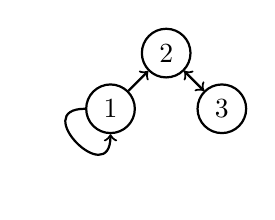
\begin{tikzpicture}[thick, main/.style = {draw, circle}] 
%\node[parameter] (nodeID) [relative position] {label};
\node[main] (1) {1};
\node[main] (2) [above right of=1] {2};
\node[main] (3) [below right of=2] {3};
\draw[->] (1) to [out=180,in=270,looseness=4] (1);
\draw[->] (1) -- (2);
\draw[->] (2) -- (3);
\draw[->] (3) -- (2);
\end{tikzpicture} \\
We can now visualize symmetry and anti-symmetry as arrows. If the relation is symmetric (i.e. if aRb then bRa), all arrows are double-sided. However, when the relation is anti-symmetric (i.e. if aRb and bRa then a=b), all arrows are single-sided. \par 
We see that it cannot be possible for an arrow to both be single- and double-sided. Therefore, the only possible graph that is symmetric and anti-symmetric consists only of loops. Similarly, any graph with both types of arrow is neither symmetric nor antisymmetric.\footnote{This section is largely based on the StackExange discussion here: \url{https://math.stackexchange.com/questions/1475354/can-a-relation-be-both-symmetric-and-antisymmetric-or-neither}.}

\part{Algorithms}

\chapter{What is an algorithm?}
An algorithm is a finite sete of well-defined instructions, in order to perform a specific task, for example
\begin{itemize}
\item to perform a computation ($x^2 + 3$, $\sum_{i=1}^{n} 4n$)
\item to solve a certain problem (Sorting, ordering)
\item to reach a certain destination (mostly in maps and graphs\footnote{The most famous problem being the travelling salesman.})
\end{itemize}
For a little bit of background history, the most ancient proof of an algorithm dates back to 2500BC, in the Babylonian era. It was used to perform a division. The name "Algorithm" comes from Al-Khwārizmī, a Persian polymath who worked on the systematic solving of quadratic equations circa 780AD. However, the most famous mathematician who worked on algorithms remains Alan Turing ($1912-1954$), who worked on breaking the Enigma Code, along with the team at Bletchley Park\footnote{If you wanna learn more or enjoy a great film, go watch \textit{The Imitation Game}.}.
\paragraph*{Specifying Algorithms}
Algorithms and their set of instructions can be presented in different ways:
\begin{itemize}
\item Natural language
\item Pseudo-code (non-specific code)
\item Programming language (specific code)
\end{itemize}
\paragraph*{Pseudo-code}
Pseudo-code is an intermediate step between natural language and code. It is precise enough that we know precisely each step but general enough that steps specific to coding (such as variable types or pointers) aren't specified.\par
This mean of writing an algorithm allows us to analyse the properties of an algorithm independently of any programming language. This is often a useful step in programming, before the implementation of any code.
\paragraph*{Typical problems}
\begin{itemize}
\item Searching Problems: finding the position of an element in a list (ordered set).
\item Sorting Problems: putting the elements of a list into an increasing order. This can be expanded to other orders and is not limited to numbers (for example, we can sort strings in alphabetical order).
\item Optimisation Problems: determining the optimal value (maximum or minimum) of a particular quantity over all possible inputs. 
\end{itemize}

\section{Searching Problems}
\paragraph*{Goal}
Given a list $S = a_{1},a_{2},a_{3},...,a_{n}$ of distinct elements and some $x$, if $x \in S$, return $i$ such that $a_{i} = x$. Else, return $-1$.
\paragraph*{Use examples}
Finding a word in a dictionary, finding a name in a student list, finding an amount in a transaction table.

\subsection{Linear Search}
\paragraph*{Definition}
The linear search algorithm goes through the list, one element at a time, from the first to the last.
\begin{algorithm}
\DontPrintSemicolon
\SetAlgoNoEnd
$i$ := 1\;
location := -1\;
\While{($i \leq n$ and $x \neq a_{i}$)}{$i = i+1$}
\If{$i \leq n$}{location := $i$}
\KwRet location
\caption{Linear Search Algorithm}
\end{algorithm}

\subsection{Binary Search}
\paragraph*{Definition}
We assume here that the input is a list of items in \textbf{increasing order}.\\
The algorithms starts by comparing the target value with the middle element of the list. If the middle element is smaller, the algorithm proceeds with the right half of the list. Otherwise, the search proceeds with the left half of the list, including the middle position.\\
We repeat this process until we have a list of size 1. If our target is equal to the element in the singleton, we return its position. Otherwise, we return 0 (or -1, depends) to indicate that the target was not located.

\subsection{Linear vs. Binary Search}
\begin{multicols}{2}
Linear search:
\begin{itemize}
\item[+]can be applied to \textit{any list}
\item[-]is not efficient
\item[-]is very slow if the element is not in the list (worst-case scenario)\par
$\ $\par
\end{itemize}
\columnbreak
Binary Search:
\begin{itemize}
\item[+]very efficient on long lists
\item[+]still efficient if the element is not in the list
\item[-]all elements must be \textit{comparable}
\item[-]list has to be \textit{sorted}
\end{itemize}
\end{multicols}
Binary search is more efficient than linear search on long lists because it removes half of the remaining list, instead of only one element per step.

\section{Sorting Problems}
\paragraph*{Goal}
Given a list $S = a_{1},a_{2},a_{3},...,a_{n}$, return a list where the elements are sorted in increasing order. (Once again, this can be extended to other orders.)\\
Sorting is important because a non-negligible part of computing resources are devoted to sorting (for example in large databases). \\
A great number of fundamentally different algorithms\footnote{It can be easier to understand the following algorithms visually. The website \url{https://mszula.github.io/visual-sorting/} is really helpful for that.} have been invented for sorting and research is still ongoing\footnote{Recently, researches have turned to deep reinforcement learning, as a means to be faster and more efficient.}.

\subsection{Selection Sort}
Selection sort makes multiple passes (or iterations) through a list of length $n$:
\begin{itemize}
\item In the first iteration, the minimum of the list is found and put into the first position by swapping the first element with the minimum element.
\item Since the first element is now guaranteed to be the smallest after the first pass, we do not take it into account anymore.
\item In the second iteration, the minimum of the list from position 2 to $n$ ($\equiv$ the second least element) is found and put into the second position by swapping the second element with the second minimum.
\item In the $k^{th}$ iteration, the minimum from position $k$ to $n$ is found and put into the $k^{th}$ position by swapping the $k^{th}$ element with the $k^{th}$ minimum.
\item And so on ...
\end{itemize}

\subsection{Bubble Sort}
Selection sort makes multiple passes through a list:
\begin{itemize}
\item In one iteration, every pair of elements that are found to be out of order are swapped (i.e. if $a_i > a_{i+1}$, we swap them).
\item Since the last element is now guaranteed to be the largest after the first iteration, in the second iteration, it doesn't need to be inspected.
\item In each iteration, one more element at the end becomes sorted and no longer needs inspection, until all elements are sorted.
\end{itemize}
We can visualise this process as the biggest elements "bubbling" all the way to the end of the list, each one after the other.

\subsection{Insertion Sort}
\begin{itemize}
\item We compare the 2$^{nd}$ element with the 1$^{st}$. If the 2$^{nd} <$ 1$^{st}$, we put the 2$^{nd}$ before the 1$^{st}$ : the first two elements are sorted.
\item Then, the 3$^{rd}$ element is compared to the 2$^{nd}$. If 3$^{rd} <$ 2$^{nd}$, it is compared to the first one and put in the correct position : the first 3 elements are sorted.
\item In each following iteration, the $j$+1$^{st}$ element is put into its correct position amongst the first $j$+1 elements.
\end{itemize}

\section{Optimisation Problems}
Optimization problems minimize or maximize some parameter over all possible inputs. 
\paragraph*{Examples}
\begin{itemize}
\item Finding a route between two cities with the smallest total distance (travelling salesman problem)
\item Determining how to encode messages using the fewest possible bits (used in .zip compression)
\end{itemize}
Interestingly enough, the mapping problem can be declined into different problems, according to your priority : fastest or shortest way, fewest connections, least elevation, ... However, these are more complex and precise, and involve more data than we will see during this course.

\subsection{Greedy Algorithms}
\ind Optimization problems can often be solved using a \textit{greedy algorithm}, which makes the "best" choice at each step. This means that it relies on making the locally optimal choice. However, this does not necessarily produce an optimal solution to the overall problem.\par
Thus, after presenting a greedy algorithm, we either prove that it is the optimal approach or find a counterexample to show that it is not.\par
One of the principles of greedy programming is that it never reconsiders its choices, contrary to the concept of \textit{dynamic programming}, which is exhaustive but ultimately guaranteed to find the solution.\par
Funnily enough, greedy algorithms sometimes not only find a bad solution, but produce the unique worst possible solution to certain problems.

\subsection{Cashier's Algorithm}
\paragraph*{Problem}
Find for any amount of $n$ cents, the least total number of coins needed using the following coins : quarters (25 cents), dimes (10 cents), nickels (5 cents) and pennies (1 cent).
\paragraph*{(Greedy) Solution}
At each step, choose the coin with the largest possible value that does not exceed the amount left. \\
\ind We see here how the choice made is local, because the algorithm does not take into account the amount that will be left after, only what is left at the moment.
\paragraph*{Proving Optimality}
We want to prove that the cashier's algorithm using quarters, dimes, nickels and pennies leads to the optimal solution.
\subparagraph*{Lemma}
If $n > 0$, then $n$ cents in change using quarters, dimes, nickels and pennies, using the fewest coins possible, 
\begin{enumerate}
\item has at most 2 dimes, at most 1 nickel, at most 4 pennies
\item cannot have 2 dimes ($2*10$\textcent) and 1 nickel ($1*5$\textcent)
\item and the total amount of change in dimes, nickels and pennies cannot exceed 24 cents.
\end{enumerate}
\subparagraph*{Proof of Lemma 1.1}
\textit{If $n > 0$, then $n$ cents in change using quarters, dimes, nickels and pennies, using the fewest coins possible, has at most 2 dimes, at most 1 nickel, at most 4 pennies.}
\begin{enumerate}[(a)]
\item Dimes, by contradiction : If we have 3 dimes, we have $3*10 = 30$ cents, which we replace by 1 quarter ($1*25$\textcent) and 1 nickel ($1*5$\textcent) = 2 coins $<$ 3 coins.
\item Nickels, by contradiction : If we have 2 nickels $= 2*5 = 10$ cents, we replace them by 1 dime ($1*10$\textcent) = 1 coin $<$ 2 coins.
\item Pennies, by contradiction : If we have 5 pennies $= 5*1 = 5$ cents, we replace them by 1 nickel ($1*5$\textcent) = 1 coin $<$ 5 coins. 
\end{enumerate}
\subparagraph*{Proof of Lemma 1.2}
\textit{If $n > 0$, then $n$ cents in change using quarters, dimes, nickels and pennies, using the fewest coins possible, cannot have 2 dimes ($2*10$\textcent) and 1 nickel ($1*5$\textcent).}\par
By contradiction : If we have 2 dimes + 1 nickel $= 25$ \textcent, we replace them with 1 quarter $= 25$ \textcent.
\subparagraph*{Proof of Lemma 1.3}
\textit{Given $n$ cents, with $n > 0$, then the total amount of change in dimes, nickels and pennies cannot exceed 24 cents.}\par
Per Lemma 1.1, we have at most 2 dimes, 1 nickel and 4 pennies, which is worth 29 cents. Per Lemma 1.2, we cannot have 2 dimes and 1 nickel. If we remove the nickel, which holds the least value, the total is 24 cents.
\subparagraph*{Proving Optimality}
Theorem : The greedy change-making algorithm for U.S. coins produces change using the fewest coins possible.
Proof by contradiction :
\begin{enumerate}
\item Assume that a solution $S'$ exists, is optimal and uses fewer coins than $S$, the solution produced by the Cashier's Algorithm.
\item let $q'$ be the number of quarters in $S'$. $q' \leqslant q$ because the cashier's algorithm picks the maximum amount of quarters.\\
Can $q' < q$? If $q' < q$, then $S'$ must have $\geqslant 25$ cents with dimes, nickels and pennies. This cannot be optimal, as per Lemma 1.3.\\
Thus, $q' = q$.
\item Since $q' = q$, $S$ and $S'$ have to change the same remaining amount of money by using dimes, pennies and nickels.
\item $d' \leqslant d$ because the cashier's algorithm takes the maximum possible amount of dimes.\\
Can $d' < d$? If $d' < d$, we need at leasts 2 extra nickels to make up for the value of the missing dime. This cannot be optimal, due to Lemma 1.1.\\
Thus, $d' = d$.
\item Since $q' = q$ and $d' = d$, $S$ and $S'$ have to change the same remaining amount of money using nickels and pennies.
\item $n' \leqslant n$, because the cashier's algorithm takes the maximum possible amount of nickels.\\
Can $n' < n$? If $n' < n$, then $S'$ would have at least 5 extra pennies to make up for the missing nickel(s). This cannot be, as per Lemma 1.1.\\
Thus, $n' = n$.
\item Since $q' = q$, $d' = d$ and $n' = n$, the remaining amount of money is the same for $S$ and $S'$. They need the same amount of pennies, leading to $p' = p$.
\item We assumed $S'$ to be optimal, so $S$ is optimal too.
\end{enumerate}
\subparagraph*{Remark}
It is important to note that we have only proven that the Cashier's Algorithm is optimal when using the American coin system. Using another set of coins does not guarantee that the greedy solution is optimal, we would have to prove that. 

\section{Matching and Stable Matching}
\paragraph*{Goal}
Pair elements from two equally sized groups considering their preferences for members of the other group so that there are no ways to improve the matching (according to the preferences).
\paragraph*{Matching}
Given a finite set $A$, a \textit{matching} of $A$ is any set of unordered pairs of \textit{distinct} elements of $A$ where any element occurs in at most one pair. (Such pairs are called \textit{independent}.) This mean that any element can appear at most once per matching set.
\paragraph*{Maximum matching}
A \textit{maximum matching} is a matching that contains the largest possible number of independent pairs.
\paragraph*{Preference list}
A \textit{preference list} $L_x$ defines for every element $x \in A$ the order in which the element prefers to be paired with another element. 
\paragraph*{Example}
Let $L_x$ be the preference list of $x$. If $L_x = [a,b,c]$, x would rather be paired with $a$, then, if not possible, with $b$, then $c$.
\paragraph*{Stability and Instability}
A matching is \textit{unstable} id there are two pairs $(a,b),(c,d)$ in the matching such that $a$ prefers $c$ over $b$ and $c$ prefers $a$ to $d$. This means that we can exchange to elements between pairs and get a better match, according to their preferences.\\
A \textit{stable} matching is a matching that is not unstable. This means that there is no pair of participants that prefer each other to their assigned match. 
\paragraph*{Example}
Given the set $A = \{Peter, Dana, Egon, Ray\}$ and the preference lists
\begin{itemize}
\item $L_{Peter} = [Dana, Egon, Ray]$
\item $L_{Dana} = [Peter, Egon, Ray]$
\item $L_{Egon} = [Peter, Dana, Ray]$
\item $L_{Ray} = [Peter, Dana, Egon]$
\end{itemize}
The matching $\{(Ray, Dana), (Egon, Peter)\}$ is unstable, because we can exchange Peter and Ray (Peter and Dana prefer each other to their assigned matches). Therefore, the matching $\{(Peter, Dana), (Egon, Ray)\}$ is stable.

\subsection{Marriage Problem}
\paragraph*{Definition}
Given a set $A$ with even cardinality (= even number of elements), partition $A$ into two disjoint subsets $A_1$ and $A_2$ with $A_1 \cup A_2 = A$ and $|A_1| = |A_2|$. A matching is a bijection from the element of one set to the element of the other set.\\
That means that pairs can only consist of one element of $A_1$ and $A_2$ each.
\paragraph*{Goal}
Find a \textit{maximum stable matching} for $A_1 \cup A_2 = A$. This is called the marriage problem.
\paragraph*{Gale-Shapley Algorithm}
This is a greedy algorithm, also known as the deferred acceptance algorithm and propose-and-reject algorithm, used to construct a stable maximum matching to answer the marriage problem. \\
\ind This algorithm is named after David Gale and Lloyd Shapley, who proved in 1982 that it is always possible to find a stable matching that answers the marriage problem. An very similar algorithm has been used since the 1950s to match medical school students to residency programs across the U.S.
\begin{algorithm}
\DontPrintSemicolon
Let $M$ be the set of pairs under construction\;
Initially $M = \emptyset$\;
\While{$\mid M\mid < \mid A_1\mid$}
{Select an unpaired $x \in A_1$\;
Let $x$ propose to the first element $y \in A_2$ on $L_x$\;
\eIf{$y$ is unpaired}
{Add the pair $(x,y)$ to $M$}
{Let $x' \in A_1$ be the element that $y$ is paired to (i.e. $(x',y) \in M$\;
\eIf{$x'$ precedes $x$ on $L_y$}{Remove $y$ from $L_x$}{Replace $(x',y) \in M$ by $(x,y)$ and remove $y$ from $L_{x'}$}}}
\caption{Gale-Shapley Algorithm}
\end{algorithm}

\section{Unsolvable Problems}
Can every problem be solved by an algorithm? This question was solved by Turing and the answer is "No". To prove that, Turing defined an unsolvable problem : the \textit{halting problem}.
\paragraph*{The Halting Problem}
$\ $\\
\ind Can we develop a procedure that takes as input a computer program and an input and determines whether the program will eventually finish running or continue to run forever?\\
\ind This problem is unsolvable because, as long as the program is running, we cannot determine if it will stop or not. More particularly, if a program halts, we can determine that it does in fact halt. But if it never halts, we cannot determine whether it will halt or not, until it halts, which it will not.
\paragraph*{Decidability}
An \textit{undecidable} problem is a decision problem for which it has been proven that no algorithm can always output a correct yes-or-no answer.

\section{Efficiency of algorithms}
In order to compare different algorithms, we have to different extreme precision degrees:
\begin{enumerate}
\item Precise count of everything involved (such as computer instructions, disk accesses, ...)\\
This means that the efficiency would be a function the size of the problem, which is inconvenient and not always well-defined.
\item "It took a few seconds on my laptop"\\
That statement is not informative. What if you run it at NASA? And what about on a Smaky 4? Then, the time and resources needed are not predictable.
\end{enumerate}
Therefore, we use another way of estimating the efficiency of an algorithm (or any procedure or computation), that is the next chapter of this class.

\chapter{Growth of Functions and Algorithm Complexity}
\paragraph*{Introduction}
Imagine that you run the following algorithm:
\begin{algorithm}
\DontPrintSemicolon
Create a list of 3000 random numbers and sort it using bubble sort (task 1)\;
Create $n$ lists of length 1500 and sort them using bubble sort (task 2)\;
Create a list of length $400*n$ and sort it using bubble sort (task 3)
\caption{$Sort\_tasks(n: integer)$}
\end{algorithm}\\
\ind We measure how much time is spent on each task depending on $n$ ($n = 1,2,3,...,20$) and we find that it is approximately
\begin{itemize}
\item[-]1000 milli-seconds for task 1, independent of $n$
\item[-]$200\cdot n$ milli-seconds for task 2
\item[-]$1.5\cdot n^2$ milli-seconds for task 3
\end{itemize}
\ind Now, we can estimate the time spent for all tasks as a function of $n$: $f(n)=1.5n^{2}+200n+1000$\par
Let $g(n)=1.5\cdot n^2$, $h(n)=200\cdot n$ and $j(n)=1000$, such that $f(n)=g(n)+h(n)+j(n)$.\par
$\ $\par
We notice that for a small value of $n$, $j(n)$ holds the most significant value. Then, $h(n)$ takes over and, ultimately, only $g(n)$ is relevant.
\paragraph*{Observation}
\ind If we generalize that observation, let $f(n)$ estimate the time to solve a problem of size $n$. If $f(n)=g(n)+h(n)+...+j(n)$ for functions g,h,...,j: $\N \to \R$. Then, the "ultimately largest" of g,h,...,j determines the behaviour of $f$ as $n$ grows.\\
\ind Let $g(n)$ be the "ultimately most relevant part" of $f(n)$. Then, the growth rate of $f(n)$ is independent of multiplicative constants in $g(n)$:
$\frac{g(m)}{g(n)}=\frac{c\cdot g(m)}{c\cdot g(n)}$\\
\ind With all of those observations, we can deduce than when considering a runtime function (here $f(n)$), we 
\begin{itemize}
\item[-]only focus on the part that grows the "fastest" (as we care about the cases where $n \to \infty$)
\item[-]forget about any multiplicative constant, because the absolute value is not important here, rather than the growth
\end{itemize}
only focus on the part that grows the "fastest" (for $n \to \infty$)
\section{Big-O Notation}
Let $f$ and $g$ be functions from the set of integers or the set of real numbers to the set of real numbers. We say that \textbf{$f(x)$ is $\mathcal{O}(g(x))$} if there exist constants $C$ and $k$ such that
\[\mid f(x)\mid \leq C\mid g(x)\mid,\ whenever\ x>k\] 
This is read as "$f(x)$ is big-$O$ of $g(x)$" or "\textit{g is an asymptotical bound (above) for f}" which is a complicated way to say that it is an upper bound (or limit) on the growth rate of $f$.\par
The constants $C$ and $k$ are called witnesses to the big-$O$ relationship. Only one pair of witnesses is needed. However, to show that $f(x)$ is \textit{not} big-$O$ of $g(x)$, we have to show that we cannot find such a pair. This can be done using a proof by contradiction.
\paragraph*{Example and common uses}
\begin{align*}
&75 \text{ is } \mathcal{O}(1) &&\text{ and }1\text{ is }\mathcal{O}(75)\\
&cos(x)\text{ is also }\mathcal{O}(1)&&\text{ and }sin(x)\text{ is }\mathcal{O}(1)\\
&1\text{ is }\mathcal{O}(x) &&\text{ but }x\text{ is not }\mathcal{O}(1)\\
&x\text{ is }\mathcal{O}(x^2) &&\text{ but }x^2\text{ is not }\mathcal{O}(x)\\
&x^2\text{ is }\mathcal{O}(x^2) &&\text{ and }x^2\text{ is }\mathcal{O}(x^3)\\
&x^2\text{ is }\mathcal{O}(6x^2+x+3) &&\text{ and }6x^2+x+3\text{ is }\mathcal{O}(x^2)&
\end{align*}
However, We rarely use $\mathcal{O}(6x^2+x+3)$ and $\mathcal{O}(75)$ because our goal is to simplify, so that it is easy to grasp the growth rate of a function.
\subsection{Big-O Estimates for Polynomials}
$\ $\\
\textbf{Theorem:} Let $f(x)=a_nx^n+a_{n-1}x^{n-1}+...+a_1x^1+A_0$ where $a_0,a_1,...,a_n$ are real numbers with $a_n \neq 0$.\par 
Then $f(x)$ is $\mathcal{O}(x^n)$. The leading term $a_nx^n$ of a polynomial dominates its growth.\par
It follows that if a polynomial is $\mathcal{O}(x^n)$, then its degree is $\leqslant n$.
\subsection{Combinations of Functions}
Many algorithms are made up of two or more separate sub-procedures. The number of steps used by a computer to solve a problem with an input of a specified size $n$ using such an algorithm is the sum of the number of steps used by these sub-procedures.
\paragraph*{Sum of functions}
$\ $\par
\textbf{Theorem:} Suppose that $f_{1}(x)$ is $\mathcal{O}(g_{1}(x))$ and that $f_{2}(x)$ is $\mathcal{O}(g_{2}(x))$. Then $(f_{1}+f_{2})(x)$ is $\mathcal{O}(g(x))$ where $g(x)=max(|g_1(x)|, |g_2(x)|)$ for all $x$.\par
\textbf{Corollary:} Suppose that $f_{1}(x)$ and $f_{2}(x)$ are both $\mathcal{O}(g(x))$. Then $(f_{1}+f_{2})(x)$ is $\mathcal{O}(g(x))$.
\paragraph*{Product of functions}
$\ $\par 
\textbf{Theorem:} Suppose that $f_{1}(x)$ is $\mathcal{O}(g_{1}(x))$ and that $f_{2}(x)$ is $\mathcal{O}(g_{2}(x))$. Then $(f_{1}\cdot f_{2})(x)$ is $\mathcal{O}(g_1(x)\cdot g_2(x))$.
\paragraph*{Transitivity}
$\ $\par
Suppose that $f(x)$ is $\mathcal{O}(g(x))$ and $g(x)$ is $\mathcal{O}(h(x))$. Then $f(x)$ is $\mathcal{O}(h(x))$.
\subsection{Useful Big-O Estimates}
\begin{itemize}
	\item{\makebox[7cm]{$n^c$ is $\mathcal{O}(n^d)$ but $n^d$ is not $\mathcal{0}(n^c)$\hfill} for $d > c > 1$}
    \item{\makebox[7cm]{$(log_bn)^c$ is $\mathcal{O}(n^d)$, but $n^d$ is not $\mathcal{O}((log_bn)^c)$\hfill} for $b>1,c,d>0$}
    \item{\makebox[7cm]{$n^d$ is $\mathcal{O}(b^n)$ but $b^n$ is not $\mathcal{O}(n^d)$\hfill} for $d>0,b>1$}
    \item{\makebox[7cm]{$b^n$ is $\mathcal{O}(c^n)$ but $c^n$ is not $\mathcal{O}(b^n)$\hfill} for $c>b>1$}
    \item{\makebox[7cm]{$c^n$ is $\mathcal{O}(n!)$ but $n!$ is not $\mathcal{O}(c^n)$\hfill} for $c>1$}
\end{itemize}
%ADD GRAPH ON GROWTH FUNCTIONS WITH EXPONENTIAL SCALE
\paragraph*{Notation}
If we want to write a big-O relation with mathematical signs, we can write $f(x) \in \mathcal{O}(g(x))$, because $\mathcal{O}(g(x))$ represents the set of functions that are $\mathcal{O}(g(x))$.
\paragraph*{Summary of Big-O Notation and nomenclature}
\begin{itemize}
	\item{\makebox[4cm]{Constant: \hfill} $\mathcal{O}(1)$}
    \item{\makebox[4cm]{Logarithmic: \hfill} $\mathcal{O}(logx)$}
    \item{\makebox[4cm]{Poly-logarithmic:\hfill} $\mathcal{O}((logx)^d),d>1$}
    \item{\makebox[4cm]{Linear:\hfill} $\mathcal{O}(x)$}
    \item{\makebox[4cm]{Linearithmic:\hfill} $\mathcal{O}(xlogx)$}
    \item{\makebox[4cm]{Polynomial:\hfill} $\mathcal{O}(x^d),d>1$}
    \item{\makebox[4cm]{Exponential:\hfill} $\mathcal{O}(b^x),b>1$}
    \item{\makebox[4cm]{Factorial:\hfill} $\mathcal{O}(x!)$}
\end{itemize}
\section{Big-Omega Notation}
Let $f$ and $g$ be functions from the set of integers or the set of real numbers to the set of real numbers. We say that \textbf{$f(x)$ is $\Omega (g(x))$} if there are constants $C > 0$ and $k$ such that \[\mid f(x)\mid \geq C\mid g(x)\mid\text{ whenever }x > k\]\par
This is read as "$f(x)$ is big-Omega of $g(x)$". Big-Omega tells us that a function grows \textit{at least as fast} as another (big-Omega is the lower bound to the growth of a function).\par 
$f(x)$ is $\Omega (g(x))$ if and only if $g(x)$ is $\mathcal{O}(f(x))$
\section{Big-Theta Notation}
Let $f$ and $g$ be functions from the set of integers or the set of real numbers to the set of real numbers. We say that \textbf{$f(x)$ is $\Theta (g(x))$} if $f(x)$ is $\mathcal{O}(g(x))$ and $f(x)$ is $\Omega (g(x))$\par
This is read as "$f(x)$ is big-Theta of $g(x)$" or $f(x)$ is of \textit{order} $g(x)$". \par 
$f(x)$ is $\Theta (g(x))$ if and only if there exist positive constants $C_1,C_2$ and $k$ such that \[C_1\mid g(x)\mid \leq \mid f(x)\mid \leq C_2\mid g(x)\mid \text{ if }x>k\]\par
When $f(x)$ is $\Theta (g(x))$ then $g(x)$ is $\Theta (f(x))$
\subsection{Big-Theta Estimates for Polynomials}
\paragraph*{Theorem}
Let $f(x)=a_nx^n+a_{n-1}x^{n-1}+...+a_1x^1+A_0$ where $a_0,a_1,...,a_n$ are real numbers with $a_n \neq 0$.\par
We already saw that the leading term $a_nx^n$ of a polynomial dominates its growth. Then $f(x)$ is of order $x^n$ or $f(x)$ is $\Theta (x^n)$.
\section{Little-o Notation}
We say that \textbf{$f(x)$ is $o (g(x))$} if \[ \lim_{x\to\infty} \frac{f(x)}{g(x)} = 0 \]
We also say the "$f$ is little-o of $g$" or "$f$ is little-omicron of $g$"
\paragraph*{Examples}
$\ $\par
$x^2$ is $\mathcal{O}(x^3)$ and it is also $o(x^3)$ as $\lim_{x\to \infty} \frac{x^2}{x^3} = 0$\par
$x^2+x+1\text{ is }\mathcal{O}(x^2)$ but it is not $o(x^2)$ as $\lim_{x\to \infty} \frac{x^2+x+1}{x^2} =1$\par 
In general, we can say that $x^n$ is $o(x^{n+1})\ \forall x \geq 0$ because $\lim_{n\to \infty} \frac{x^n}{x^{n+1}} =0$
\subsection{Little-o and Big-O}
If $f(x)$ and $g(x)$ are functions such that $f(x)$ is $o(g(x))$, then $f(x)$ is $\mathcal{O}(g(x))$\par 
However, if $f(x)$ is $\mathcal{O}(g(x))$, it does not necessarily follow that $f(x)$ is $o(g(x))$.\par 
$f(x) \in o(g(x)) \implies f(x) \in \mathcal{O}(g(x))$
\paragraph*{Theorem: finite limit and Big-O}
$\ $\par 
If $\lim_{x\to \infty} \frac{f(x)}{g(x)}=c$ with $c$ finite, then $f(x) \in \mathcal{O}(g(x))$\par 
This is proved as follows:
\begin{enumerate}
\item $\forall \varepsilon >0, \forall x>k, |\frac{f(x)}{g(x)} -c| \leqslant \varepsilon$ (definition of the limit)
\item $|\frac{f(x)}{g(x)}| \ =\ |\frac{f(x)}{g(x)} -c +c| \ \leqslant \ |\frac{f(x)}{g(x)} -c| + |c|\ =\ \varepsilon+|c|$
\item We take $\varepsilon = 1$ (but we can pick any value we want). $|\frac{f(x)}{g(x)}|\ \leqslant \ 1+|c|$.
\item It follows that $|f(x)|\ \leqslant \ (1+|c|)\ |g(x)|$
\end{enumerate}
\section{Back on Algorithm Complexity}
Given an algorithm, we want to measure how efficient it is for solving a problem given an input of a particular size (\textit{computational complexity}). For that, we differentiate two types:
\begin{itemize}
\item \textbf{Time complexity}: How much time is needed to solve the problem of an input of a given size
\item \textbf{Space complexity}: How much computer memory is used
\end{itemize}
Understanding complexity is important to understand whether it is practical to use an algorithm for inputs of a particular size and to compare the efficiency of different algorithms designed to solve the same problem.\par 
This course focuses only on time complexity, which corresponds to the number of operations performed is the algorithm is sequential. To describe that, we will use big-O and big-Theta notation. We will also ignore implementation details, because that is too complicated for the scope of this course.\par 
To determine time complexity, we need to determine the number of basic operations (such as addition, multiplication, comparisons, swaps, etc.) while ignoring details like the "house keeping" aspects of the algorithm (storing a value in a variable, incrementing a variable, etc.).\par 
\subsection{Worst-case Time Complexity}
Sometimes, the number of operations depends on the exact configuration of the input (a position in a list, ...), which is why we focus on the \textit{worst-case} time complexity of an algorithm. This provides an upper bound on the number of operations depending on the input size. It is generally much more difficult to determine the \textit{average case} time complexity, which is the average number of operations for all inputs of a particular size.
\subsection{Complexity of important algorithms}
Worst case complexities
\begin{itemize}
\item Linear Search: $\Theta (n)$
\item Binary Search: $\Theta (log_2(n))$
\item Bubble Sort: $\Theta (n^2)$
\item Insertion Sort: $\Theta (n^2)$
\item Selection Sort: $\Theta (n^2)$
\end{itemize}
\subsection{Effect of Complexity}
A single operation takes around $10^{-9}$ seconds, meaning we perform 1 billion bit operations per second (on a processor running at 1 GHZ).\par 
The bigger the time complexity of an algorithm, the longer it takes to run on any computer. For example, an algorithm that is $\Theta (n\cdot log(n))$ takes $2\cdot 10^{-2}$ seconds for an input of size $10^6$ but an algorithm of complexity $n^2$ would take 17 minutes. That difference does not seem like much when we only use algorithms with small input sizes in our daily lives but is is crucial in companies using large databases.
\subsection{Complement: Decreasing Complexity}
This was not seen during class, but I thought it interesting to add as a complement. \\
Consider the following problem: \par 
Given a sequence $(a_n),n\in\N$, you want to find a value $j$ such that there exists an element $a_i$ of the sequence that is in a given range $[a,b]$ for $i<j$. This means that, the greater the value of $b-a$, the less you will have to compute the sequence to find a value in that range.\par 
For example, if we take the sequence $a_n = n\cdot sin(n)$, we will have $(a_n)$ between $n$ and $-n$. If we want to get a value between a small range $[a,b]$, we will have to compute a lot of values of $(a_n)$. However, for a bigger range, it is much more likely that there will be a value within that range early on. In this example, the complexity is $\frac{1}{b-a}$, which is decreasing.

\chapter{Induction, Recursion}
Induction and recursion are different approaches to proving 
results and solving problems.\par
They both in the first place rely on the ability to achieve the 
desired result for the smallest possible version of the problem 
at hand.\par
Induction extends this ability to problems of any size, while recursion reduces a problem of any size to the smallest 
possible ones.
\paragraph*{Definition}
A \textit{recursive definition} of a function $f$ with the set of non-negative integers as its domain consists of two steps:\\
\ind Basis step: specify the value of $f$ at 0.\\
\ind Recursive step: Give a rule for finding its value at $f(n)$, with $n$ an integer, from its values at smaller values of $n$.\\
A function $f(n): \Z_{\geqslant 0} \to \R$ is the same as a sequence $a_0,a_1,a_2,...$ where $a_i$ is a real number for every $i \in \Z_{\geqslant 0}$\footnote{aka a "\textit{suite}" $(a_n)$}.\\
Recursive functions can be seen as a more generalized version of recursive sequences, because their domain of definition is not limited to integers.
\paragraph*{Example}
The factorial function $n!$ can be defined recursively as $f(0)=1$ (basis step) and $f(n+1)=(n+1)\cdot f(n)$.\\
The Fibonacci numbers are defined as\\
$f_{0}=0$\\$f_{1}=1$\\$f_{n}=f_{n-1}+f_{n-2}$
\section{Induction}
Mathematical induction can be expressed as the rule of inference, for $n\in\Z^+$
\[(P(1)\land\forall k(P(k)\to P(k+1)))\to\forall nP(n)\]
This means that $P(1)\to P(2)\to P(3)\to\ldots$.
\subsection{Proving mathematical induction}
Firstly, express the statement you want to prove in the form of "$\forall n\geq b,P(n)$ (for a certain $b$).\par
Then, evaluate your basis step. This means that you have to prove your statement for the aforementioned $b$. If you chose $P(n)$ for all positive integers, then $b=1$. If you stated $P(n)$ for all non-negative integers, then $b=0$. \par 
Thirdly, prove the induction. There, we assume that $P(n)$ is true for an arbitrary $n$ and we want to show that it implies that $P(n+1)$ is true. You have to prove $P(n+1)$ by using $P(n)$.\par 
Finally, we can conclude that by mathematical induction, $P(n)$ is true for all $n\geq b$.
\subsection{Strong induction}
To prove a statement $P(n)$, we can use induction a bit differently. The basis step is the same but instead or proving $p(n)\to P(n+1)$, we prove that $[P(1)\land P(2)\land\ldots\land P(k)]\to P(k+1)$.
\section{Recursion on Strings}
\paragraph*{Definition}
The set $\Sigma^{*}$ of strings over the alphabet $\Sigma$ is defined inductively by\par
Basis step: $\lambda \in \Sigma^{*}$ (where $\lambda$ is the empty string)\par
Inductive step: If $w \in \Sigma^{*}$ and $x \in \Sigma$ ($x$ is a character), then $wx \in \Sigma^{*}$\\
The recursive definition of $l(w)$, the function returning the length of the string $w$ is:\par
Basis step: $l(\lambda)=0$\par
Recursive step $l(wx)=l(w)+1$ if $w\in \Sigma^{*}$ (a sequence of characters) and $x \in \Sigma$ (a single character).
\paragraph*{Theorem}
$l(xy)=l(x)+l(y)$, where $x$ and $y$ belong to $\Sigma^{*}$, the set of strings over the alphabet $\Sigma$.\\
Here the induction proof is not over $P(n)$ but over $P(x,y)$. In order to do the proof, we have to focus on one parameter only: $P(x,y)$ becomes $P(y)= \forall x \in \Sigma^{*}, l(xy)=l(x)+l(y)$
\begin{itemize}
\item Basis step: we always use $\lambda = ""$ as the base case for strings\\
$\forall x \in \Sigma^{*}, l(x\lambda) = l(x)+l(\lambda) = l(x)$
\item Inductive step: $P(y) \to P(yc)$ is true $\forall c \in \Sigma$ (c is a character)\\
$P(yc) = \forall x \in \Sigma^{*},\ l(xyc) = l(xy) + 1$ (by definition of recursive $l$)\\
$\hspace*{100pt} = l(x) + l(y) +1$ (by induction hypothesis)\\
$\hspace*{100pt} = l(x) + l(yc)$ (by definition of recursive $l$)
\end{itemize}
\section{Recursive Algorithms}
An algorithm is called \textit{recursive} if it solves a problem by reducing it to an instance of the same problem with a smaller input.\par
For the algorithm to terminate, the instance of the problem must eventually be reduced to some initial case for which the solution is known.\par 
The first step is to find a recursive definition of the problem (or function).\par 
The second step is to write a method (using pseudocode first) that solves the problem using the recursive definition
\paragraph*{Example}
To compute the factorial $n!$ of an integer $n \geqslant 0$, we do the following:
\begin{enumerate}
\item[-] Step 1: recursive definition of factorial function $n!$
\item[-] Step 2: recursive procedure for computation of factorial
\end{enumerate}
\begin{procedure}
\caption{factorial(n: non-negative integer)}
\DontPrintSemicolon
\SetAlgoNoEnd

\eIf{$n=0$}{\KwRet 1}{\KwRet $n\cdot factorial(n-1)$}
\end{procedure}
\subsection{Intermezzo: Call Stack}
A call stack stores information about the active subroutines of a program and works kind of like a pile of books: 
\begin{itemize}
\item[-] the caller pushes the return address onto the stack
\item[-] the called subroutine, when it finished, pulls or pops the return address off the call stack and transfers control to that address
\end{itemize}
An active subroutine is one that has been called but is yet to complete execution, after which control is handed back to the caller (or point of call). One common error in programming is that of \texttt{StackOverflow Error}. This means that all the space allocated for the call stack has been consumed, generally by an infinitely recursive function.\par 
\paragraph*{Example}
If we take once again our example of the recursive factorial with a value of $n=6$, we first add to the call stack \texttt{factorial(6)}. The function becomes \texttt{return 6$\cdot$factorial(5)} and then \textit{calls} \texttt{factorial(5)}. This goes on until \texttt{factorial(2)} becomes \texttt{return 2$\cdot$factorial(1)}. This finally calls \texttt{factorial(1)}, which returns 1. The control is then return to \texttt{return 2$\cdot$factorial(1)} and so on, until the stack is empty.
\section{Recursion and Iteration}
We can evaluate a recursively defined function using a:
\begin{itemize}
\item Recursive algorithm: applies directly the recursive definition until the base is reached
\item Iterative algorithm: starts with the base cases and applies the recursive definition to compute the function for larger values
\end{itemize}
\paragraph*{Example}
Our goal is to compute $a^n$ where $a \in \R^{*}$ and $n>0$\par 
\begin{procedure}
\caption{power recursive(a, n)}
\DontPrintSemicolon
\SetAlgoNoEnd
\eIf{n=0}{\KwRet 1}{\KwRet $a\cdot power(a,n-1)$}
\end{procedure}
\begin{procedure}
\caption{power iterative(a, n)}
\DontPrintSemicolon
\SetAlgoNoEnd
res = 1\;
\For{$i=1$ \KwTo $n$}{res = a*res}
\KwRet res
\end{procedure}
\subsection{Divide and Conquer}
Strategy for solving a problem of size $n$:
\begin{enumerate}
\item \textbf{Divide}:
\begin{itemize}
\item if $n>1$: divide the problem of size $n$ into 2 (almost) equally sized subproblems
\item else: solve the problem of size 1 directly
\end{itemize}
\item \textbf{Conquer}: solve the subproblems in the same way (recursively)
\item \textbf{Merge}: merge the subsolutions into an overall solution
\end{enumerate}
\paragraph*{Example: Binary Search}
Assume we have $a_1,a_2,...,a_n$ an increasing sequence of integers. We are looking for an element $x$ in this sequence.
\begin{enumerate}
\item Divide:
\begin{enumerate}
\item if $n>0$: find the middle element $a_m$ of the list
\item else: the sequence is empty, $x$ is not in the list
\end{enumerate}
\item Conquer:
\begin{enumerate}
\item if $x=a_m$: we have found the element $x$ and can stop the search here
\item if $x<a_m$: search the left half (up to $a_{m-1}$)
\item if $x>a_m$: search the right half (from $a_{m+1}$ up)
\end{enumerate}
\end{enumerate}
The pseudocode for that algorithm would look something like this:
\begin{procedure}
\caption{binary search(x,l,r: integers)}
\DontPrintSemicolon
\SetAlgoNoEnd
\eIf{$l>r$}{\KwRet -1}{m:=$\lfloor (l+r)/2\rfloor$\;
\If{$x<a_m$}{$binary\_search(x,l,m-1)$}\ElseIf{$x>a_m$}{$binary\_search(x,m+1,r)$}\Else{\KwRet $m$}}
\end{procedure}
We can see that each time, the length $n$ of the sequence is divided by 2. This corresponds to a complexity of $\mathcal{O}(log(n))$.\par 
Sorting algorithms like Bubble Sort previously had a complexity$\in \Theta(n^2)$. Now, Merge Sort is significantly faster in sorting a sequence $S$ of size $n$.
\subsection{Merging two sorted lists}
Traverse the two lists simultaneously from left to right. Always take the smaller element of the two lists.
\begin{procedure}
\caption{merge($L_1,L_2$: sorted lists)}
\DontPrintSemicolon
\SetAlgoNoEnd
$L$ := empty lists
\While{$L_1$ and $L_2$ are both non-empty}{remove smallest of first elements of $L_1$ and $L_2$ from its list\;
put it at the right end of $L$\;
\If{this removal make one list empty}{remove all elements from the other list and append them to $L$}}
\KwRet $L$
\end{procedure}\\
The worst case for this procedure is when the two list alternate, because we have to keep comparing elements. This means $|L_1|+|L_2|-1$ comparisons.
\paragraph{Merge Sort Complexity}
Merge sort works as follows:\\
\begin{procedure}
\caption{mergesort($L=a_1,a_2,...,a_n$)}
\DontPrintSemicolon
\SetAlgoNoEnd
\If{$n>1$}{
$m := \lfloor n / 2 \rfloor$\;
$L_1 := a_1,a_2,...,a_m$\;
$L_2 := a_{m+1},a_{m+2},...,a_n$\;
$L := merge(mergesort(L_1),mergesort(L_2))$}
\end{procedure}\\
Merge sort works in layers ($k$). We set $n=2^m \Leftrightarrow m=log_2(n)$.\par 
At $k=0$, we have 1 list of length $2^m=n$.\par 
At $k=1$, we have 2 lists of length $2^{m-1}=\frac{n}{2}$.\par
...\par
At $k=m$, we have $2^m$ lists of length $1$. \\
Now, we go backwards and merge lists\par
At $k=m$ we need to do $2^{m-1}$ merges between lists of size 1, with a complexity of range $1+1-1=2-1$\par 
At $k=m-1$, we have $2^{m-1}$ lists and do $2^{m-2}$ merges between lists of size 2, with a complexity range of $2+2-1=4-1$\par 
If we generalize, for any k, we have $2^k$ lists and $2^{k-1}$ merges to do, which is a complexity of $2^{m-k} + 2^{m-k} -1 = 2^{m-k+1} -1 = 2^{m-(k-1)} -1$\\
The total complexity is 
\begin{align*}
\sum_{k=1}^{m} \overbrace{2^{k-1}}^{nb.\ merges} \cdot (2^{m-(k-1)} -1) &= \sum_{k=1}^m (2^{m-(k-1)+(k-1)}-2^{k-1})\\
&= m\cdot 2^m - \sum_{k=1}^{m} 2^{k-1}\\
&= m\cdot 2^m - \underbrace{\dfrac{1-2^m}{1-2}}_{negligible} \in \mathcal{O}(m\cdot 2^m) = \mathcal{O}(nlog_2(n))
\end{align*}

\section{Number Representation}
\subsection{Representation of Integers}
In general, we use decimal notation to represent integers. For example, 965 represents 9 hundreds + 6 tens + 5 ones or $9\cdot 10^2+6\cdot 10^1+5\cdot 10^0$. We also call this \textit{base 10} notation.\par 
However, different contexts call for different representations. For example, computers use binary numbers or base 2 notation.\par 
We can represent numbers using any base $b$ where $b$ is a positive integer greater than 1. As an example, the ancient Mayans used a base 20 and the ancient Babylonians used base 60.\par 
The ones we will use most in computing and communications are bases $b=2$(binary), $b=8$(octal) and $b=16$(hexadecimal).
\subsection{Base \texorpdfstring{$b$}{b} representation}
For a base $b$ ($b$ > 1) and any positive integer $n$, there is a unique choice of 
\begin{itemize}
\item $k$, a non-negative integer
\item $a_0,a_1,...,a_k$ integers with $0 \leq a_j \leq b-1$ and $a_k \neq 0$
\end{itemize}
\[n=a_kb^k+a_{k-1}b^{k-1}+...+a_1b+a_0\]
The $a_j$ coefficients are called the base $b$ digits of the representation
\subsection{Base \texorpdfstring{$b$}{b} expansion of \texorpdfstring{$n$}{n}}
For a positive integer $n$, when $n=a_{k}b^{k}+a_{k-1}b^{k-1}+...+a_1b+a_0$, we write \[(a_k a_{k-1} ... a_1 a_0)_b \] the representation in base $b$ of $n$.
\subsection{Common Bases}
\begin{itemize}
\item{\makebox[6cm]{Decimal Expansion\hfill} base 10}
\item{\makebox[6cm]{Binary Expansion\hfill} base 2}
\item{\makebox[6cm]{Octal Expansion\hfill} base 8}
\item{\makebox[6cm]{Hexadecimal Expansion\hfill} base 16}
\end{itemize}
\paragraph*{Example}
$(17)_{10} = 1\cdot 10^1 + 7\cdot 10^0 = (10001)_2 = 1\cdot 2^4 + 1\cdot 2^0 = (21)_8 = 2\cdot 8^1 + 1\cdot 8^0 = (11)_{16} = 1\cdot 16^1 + 1\cdot 16^0$
\paragraph*{Binary Expansions}
Most computers represent integers and do arithmetic with binary expansion of integers, with 0 and 1 being the only digits used (representing true and false).
\paragraph*{Octal Expansions}
The octal expansion uses the digits $\{0,1,2,3,4,5,6,7\}$
\paragraph*{Hexadecimal Expansions}
$\ $\par
Because we only have the digits 0 to 9 but need 16 digits for the representation, we use letter to expand our usual digits set. Thus $10=A, 11=B, 12=C, 13=D, 14=E$ and $15=F$ (and 16 is simply $1\cdot 16^1$ because the digits must be smaller than the base).\par 
The digits are then $\{0,1,2,3,4,5,6,7,8,9,A,B,C,D,E,F\}$
\subsection{Constructing a base \texorpdfstring{$b$}{b} expansion}
What is $(n)_10$ in binary notation?\par
One algorithm would be to first find $k$ and then work down to find $a_k$ then $a_{k-1}$ etc. This would be a version of the cashier's algorithm but with the base instead of the coin values.\par 
Algorithm:
\begin{itemize}
\item[-] Find $k$ by computing successive powers of $b$ until you find the smallest $k$ such that $b^k \leq n < b^{k+1}$
\item[-] For each value of $i$ from 0 to $k$:
	\begin{itemize}
	\item[-] Set $a_{k-1}$ to be the largest number between 0 and $b-1$ for which $a_{k-1}\cdot b^{k-1} \leq n$
	\item[-] Update the current remaining value $n := n-a_{k-1}\cdot b^{k-1}$
	\end{itemize}
\end{itemize}
\subsection{Bases and Divisibility}
When $k > 0$: 
\begin{align*}
n &= a_kb^k + a_{k-1}b^{k-1} + ... + a_1b + a_0\\
  &= b(a_kb^{k-1} + a_{k-1}b^{k-2} + ... + a_1) + a_0
\end{align*}
If $a$ and $b$ are integers with $a \neq 0$, then $a$ divides $b$ if there exists an integer $c$ such that $b=a\cdot c$ or $\dfrac{b}{a}$ is an integer
\paragraph*{Notation}
The notation $a \mid b$ denotes that $a$ divides $b$. If $a$ does not divide $b$, we write $a \nmid b$.
\subsection{Algorithm}
\paragraph*{Theorem}
If $a$ is an integer and $d$ is a positive integer, then there are unique integers $q$ and $r$ (with $0 \leq r < d$) such that $a=d\cdot q + r \Leftrightarrow \dfrac{a}{q} = d+\dfrac{r}{q}$\par
$d$ is called the \textit{divisor}.\par
$a$ is called the \textit{dividend}.\par
$q$ is called the \textit{quotient}.\par
$r$ is called the \textit{remainder}.\\
For $a=d\cdot q + r$ we write:\par 
$q = a$ \textbf{div} $d\ \ \ \ \ \ $div is a function: \textbf{div}:$\Z\times\Z^+ \to \Z$\par 
$r = a$ \textbf{mod} $d\ \ \ \ $mod is a function: \textbf{mod}:$\Z\times\Z^+ \to \N$ \par 
\paragraph*{Base $b$ Expansion Algorithm}
$\ $\\
\begin{procedure}
\caption{base b expansion($n,b$: positive integers)}
\DontPrintSemicolon
\SetAlgoNoEnd
$q := n$\;
$k := 0$\;
\While{$q\neq 0$}{
$a_k := q \pmod{b}$\;
$q := q div b$\;
$k := k+1$\;}
\KwRet ($a_{k-1},...,a_1,a_0$)
\end{procedure}
{($a_{k-1},...,a_1,a_0$)} is the base $b$ expansion of $n$. The digits are the remainders of the division given by q $\pmod{b}$.
\paragraph*{Example}
We are trying to compute $(12'345)_8$
\begin{align*}
12'345 &= 8\cdot \overbrace{1'543}^{remainder} + 1\\
\overbrace{1'543} &= 8\cdot 192 + 7\\
192 &= 8\cdot 24 + 0\\
24 &= 8\cdot 3 + 0\\
3 &= 8\cdot 0 + 3\\
(30071)_8 &= 12'345
\end{align*}


\part{Counting}
\chapter{Basic Counting Principles}
\section{Counting Subsets of a finite set}
We use the product rule to show that the number of different subsets of a finite set $S$ is $2^{|S|}$.\\
Proof:
\begin{itemize}
\item When the elements of S are listed in an arbitrary order, there is a one-to-one correspondence between subsets of S and bit strings of length $|S|$.
\item When the $i^{th}$ element is in the subset, the bit string has a 1 in the $i^{th}$ position and a 0 otherwise.
\item By the product rule, there are $2^{|S|}$ such bit strings, and therefore $2^{|S|}$ subsets.
\end{itemize}
\paragraph*{Example}
$A = \{a,b,c,d\}$\\
We can represent any subset of A by a bitstring of $n$ times 0 and 1. Here, $1101$ corresponds to the subset $\{a,b,d\}$ of A.\\
We can see that there are $2\times 2\times ... \times 2 = 2^n$ possible bitstrings. Hence, the cardinality of the power set of $S$ is $2^n$.
\section{Counting functions}
How many functions are there from a set with $m$ elements to a set with $n$ elements?\par 
Let $m = \{0,1,2,...,m-1\}$. Each element of $m$ can be mapped to any element of $n$, meaning there are $n$ possibilities for every element of $m$, which leads to $n\times n\times ...\times n = n^m$ possibilities $=n^m$ functions.
\subsection{Counting one-to-one functions}
\paragraph{Injective functions}
$ $\\
How many \textit{injective functions} are there from a set with $m$ elements to a set with $n\geq m$ elements?\par 
Let $m= \{0,1,2,...,m-1\}$. The first element can be mapped to $n$ elements of $n$. The second can be mapped to $n-1$ elements of $n$, because the functions are injective and one element of $n$ is already mapped to by one element of $m$. This goes on until the $m^{th}$ element of $m$ can be mapped to the only remaining element of $n$. Thus, our possibilities are $n\cdot (n-1)\cdot (n-2)\cdot\ldots\cdot (n-m)=\frac{n!}{(n-m)!}$.
\paragraph{Surjective functions}
$ $\\
How many \textit{surjective functions} are there from a set $A$ with $m$ elements to a set $B$ with $n\geq m$ elements?\par 
We work backwards here. Every element of $B$ must be mapped to at least one element of $A$. This is not possible if $m<n$. Therefore, we need $m=n$. There, the first element of $B$ has $n$ choices, the second has $n-1$, and so on. Therefore, there are $n!$ surjective functions.
\section{The Sum Rule}
If $S_1,S_2,...,S_n$ are finite \textbf{disjoint} sets, then $|\bigcup_{i=1}^{n} S_i| = |S_1| + |S_2| + ... + |S_n|$.
\paragraph*{Example}
Counting Passwords: Each user on a computer system has a password, which is 6 to 8 characters long, where each character is an uppercase letter or a digit. Each password must contain at least one digit. \\
How many possible passwords are there?\par 
To do this, we separate the passwords into three distinct sets $P_6,P_7,P_8$ depending on the number of characters. Then, for each set, we count all the possibilities minus the possibilities without any digit.\\
This is counted as $P_6=(26+10)^6-26^6$, $P_7=36^7-26^7$, $P_8=36^8-26^8$. Then, because the three sets are disjoint, we add them: $P=P_6+P_7+P_8$
\section{The Substraction Rule}
Let $A$ and $B$ be two finite sets. Then, $|A\cup B|=|A|+|B|-|A\cap B|$. This is the \textbf{inclusion-exclusion principle}.
\paragraph*{Example}
How many bit strings of length 8 either start with 1 bit or end with the two bits 00?\par 
$|\underbrace{\text{start with 1}}_{\text{1xxxxxxx}}|+|\underbrace{\text{end with 00}}_{\text{xxxxxx00}}|-|\underbrace{\text{both}}_{\text{1xxxxx00}}| = 1\cdot 2^7+2^6\cdot 1\cdot 1-1\cdot 2^5\cdot 1\cdot 1 = 160$
\section{Permutations, combinations, repetitions}
It is important to note that while this distinction is not made in the course, i differential partial permutations from permutations, because this is what I was taught and because it make more sense to me. 
\subsection{Partial Permutations}
In French, "arrangement", a permutation is taking $k$ distinct element among $n$ distinct elements and putting them in a \textbf{particular order}. The number of permutations is 
\[(A^n_k=)P(n,k) = n(n-1)(n-2)...(n-k+1)=\frac{n!}{(n-k)!}\] 
\subsection*{Partial Permutations with repetitions}
If, among $n$ distinct elements, we pick $k$ elements (distinct or not) and sort them in a \textbf{particular order}, the number of permutations with repetitions is
\[\overline{A^n_k}=n^k\]
This is because for each element we pick, we have $n$ choices. This is $n$ choices $k$ times $=n\cdot n\cdot ...\cdot n=n^k$.
\subsection{Permutation}
If we sort $n$ distinct elements in a \textbf{particular order} (and not only part of those $n$ elements), we form a simple permutation. The formula is 
\[P_n = n!\]
\subsection*{Permutation with repetitions}
If we sort in a \textbf{particular order} $n$ elements that include $n_1$ identical elements of type 1, $n_2$ identical elements of type 2, ... ($n_1+n_2+...+n_p=n$), we do a permutation with repetitions. The formula is
\[\overline{P}(n_1,n_2,...,n_p)=\frac{n!}{n_1!n_2!...n_p!}\]
\subsection{Combinations}
If, among $n$ distinct elements, we pick $k$ distinct elements ($k\leq n$) and sort them in \textbf{no particular order}, the number of combinations is
\[C^n_k = \begin{pmatrix}n\\k\end{pmatrix} = \frac{P(n,k)}{k!} = \frac{n!}{k!(n-k)!}\]
Here, we count the number of possible permutations and divide it with the number of possible orders. What remains is the number of permutations with no order.\par 
$C^n_k$ or $C(n,k)$ is also read as "choose $k$ from $n$", which is self-explanatory.
\subsection*{Combinations with repetitions}
If, among $n$ distinct elements, we pick $k$ elements (distinct or not) and sort them in \textbf{no particular order}, the number of combinations with repetitions is
\[\overline{C^n_k} = \frac{(n+k-1)!}{k!(n-1)!} = \begin{pmatrix}n+k-1\\k\end{pmatrix}\]
This is directly related to the "stars and bars" counting method.
\subsection{Stars and bars}
A combination with repetitions can be modeled as categories representing each distinct element to choose from, separated each by a bar (so $n-1$). The number of times we choose that element are stars that we put between the bars (with $k$ stars in total). \par
If we take a step back, instead of seeing it as stars between bars, we can see it as bars between stars. Therefore, the possibilities are counted as the placement possibilities for the bars.\par 
For $k$ elements from $n$ distinct ones, the formula is $C(n+k-1,n-1) = \begin{pmatrix}n+k-1\\n-1\end{pmatrix} = \begin{pmatrix}n+k-1\\k\end{pmatrix}$, the number of ways to place $n-1$ bars.
\paragraph*{Stars and bars: equation edition}
The stars and bars method is particularly useful with equations of the form $x_1+x_2+...+x_n\leq y$. The methodology for that sort of question is as follows:
\begin{enumerate}[nosep]
\item If some $x_i$ have a value or $x_i\leq a_i$, introduce the variable change $y_i = x_i-a_i$. The sum will then be minus all those $a_i$.
\item If the equation is $<y$, rewrite it as $\leq y-1$.
\item If the equation is not $=y$, introduce a "dummy variable" $x_{n+1}$, such that $x_1+x_2+...+x_n+x_{n+1}=y$.
\item Finally, use the stars and bars method : if there is no dummy variable, $C\begin{pmatrix}n+y-1\\y\end{pmatrix}$, and if there is, $C\begin{pmatrix}(n+1)+y-1\\y\end{pmatrix}$
\end{enumerate}
\section{Pigeonhole Principle}
If $k+1$ elements are placed in $k$ boxes ($k>0$), then at least one box contains 2 or more objects.
\subsection{Generalised Pigeonhole Principle}
If $N$ objects are placed into $k$ boxes, then at least one box contains at least $\lceil N/k\rceil$ objects.
\subsection{Inverse Pigeonhole Principle}
If we have $k$ boxes, we need $(N-1)\cdot k+1$ objects so that at least one box contains at least $N$ objects.

\chapter{Probability}
\section{Expected Value}
The expected value or "espérance" in French is what result you expect to get for the random variable $X$ over the space $S$. It's a bit like an average outcome. However, it may not be included in the space. For example, if I throw a pentagonal die\footnote{Singular for dice (I didn't know it either).} (D7), the expected value would be 3.5, although you cannot get a decimal value on a die.\par 
The expectancy is calculated as
\[E(X)=\sum_{s\in S}p(s)X(s)\]
The expected value is linear, meaning that $E(X_1+X_2+...+X_n)=E(X_1)+E(X_2)+...+E(X_n)$ and $E(aX+b)=aE(X)+b$. This is useful if two random variables' expected values differ from a constant. We can have a kind of "changement de variable" as $E(Y)=E(X)+c$.
\section{Variance}
The variance is "the expected value of the squared deviation from the mean of a random variable\footnote{Thanks Wikipedia \url{https://en.wikipedia.org/wiki/Variance}}". This is not very clear but to me, it just means that the variance is how much you can expect to vary from the expected value. However, this is not mathematical, just a way to visualise better.\par 
The variance of a random variable $X$ over a sample space $S$ is computed as 
\[V(X)=\sum_{s\in S}(X(s)-E(X))^2\cdot p(s)\]
However, that can be a hassle to calculate. The other formula for the variance is $V(X)=E(X^2)-E(X)^2$, and id $E(X)=\mu$, then $V(X)=E((X-\mu)^2)$.
\section{Bernoulli Trials}
Bernoulli trials are a probability law for an event that has two outcomes (True/False, heads/tails, red/green, ...) one considered as a "success" and the other as a "failure\footnote{We are still proud of you, kiddo.}". This is the same as saying that the universe $U$ has two elements ($\{0,1\}$ for example). The random variable $X$ has the value 1 if one event succeeds and 0 if it doesn't. We have $p$ the probability of success and $q$ the probability of failure ($p+q=1$). \par 
The probability of $k$ successes over $n$ (independent) trials is 
\[p(X=k)=C(n,k)\cdot p^k\cdot q^{n-k}\]
\paragraph{Expected value}
The expected value of $n$ Bernoulli trials with a probability $p$ of success is $E(X)=n\cdot p$.
\paragraph{Variance}
The variance of $n$ Bernoulli trials is $V(X)=np(1-p)$.
\section{Conditional Probability}
Conditional probability is the probability of an event $A$ happening knowing that an event $B$ has happened. We write $P(A\mid B)=$ "probability of $A$ knowing $B$".\par 
This is usually computed as $P(A\mid B)=\frac{P(A\cap B)}{P(A)}$.
\subsection{Bayes' Theorem}
Bayes' theorem is useful when we have no information about the intersection of the two events. Instead, we compute
\[P(A\mid B)= \frac{P(B\mid A)P(A)​}{P(B)}\]
\subsection{Generalized Bayes' Theorem}
If $A_1\cup 1_2\cup\ldots\cup A_n=U$ and $\forall i,j\ A_i\cap A_j=\emptyset$, then 
\[P(A_k\mid B)=\frac{P(B\mid A_k)P(A_k)}{P(B)}\]
This is useful when the space is divided in multiple incompatible events.
 

%“Every time I climb Mount Everest, I eat a pizza.”
%— Topology professor on vacuous truth
%https://mathprofessorquotes.com/

\end{document}
